\documentclass[english]{panikzettel}

\usepackage{tikz}
\usetikzlibrary{arrows,automata,shapes}

\tikzstyle{every task} = []
\tikzstyle{every gateway} = []
\tikzstyle{every sequence} = []
\tikzstyle{every message} = []
\tikzstyle{every association} = []
\tikzstyle{every event} = []

\tikzstyle{task} = [rectangle, draw, black,
                      minimum width=4em, minimum height=2em,rounded corners,align=center,every task]

\tikzstyle{gateway} = [diamond, draw, black,inner sep=0pt,minimum width=1.5em, minimum height=1.5em,every gateway]
\tikzstyle{sequence} = [->,>=triangle 45,every sequence]
\tikzstyle{message} = [o->,dashed,>=open triangle 45,every sequence]
\tikzstyle{association} = [->,densely dotted,>=angle 45,every association]
\tikzstyle{event} = [circle,minimum width=2em, minimum height=2em,draw,every event]
\tikzstyle{end event} = [event,ultra thick,every event]
\tikzstyle{intermediate event} = [event,double,every event]

\usepackage{listings}
\lstset{escapechar=\&,
        stringstyle=\ttfamily,
        keywordstyle=\bold,
        emph={Action, Precond, Effect, Op},
        emphstyle={\bfseries}
    }

\tikzset{
    place/.style = {circle,fill=none,draw=black,text=black},
    trans/.style = {rectangle,fill=none,draw=black,text=black},
    activ/.style = {rounded corners, rectangle,fill=none,draw=black,text=black,minimum width=0.6cm, minimum height=0.6cm},>=stealth',shorten >=1pt,auto,node distance=1cm,thick,
    initial text = \textcolor{red}{}
}

\usepackage{array}
\usepackage{multirow}
\newcolumntype{L}{>{$}l<{$}}

\usepackage{nicefrac}

\title{Business Process Intelligence Panikzettel}
\author{Caspar Zecha, Philipp Schröer, Luca Oeljeklaus}

\begin{document}

\maketitle

\tableofcontents

\section{Introduction}

This Panikzettel is about the lecture Business Process Intelligence by Prof.\ van der Aalst held in the summer semester 2018.

This Panikzettel is Open Source. We appreciate comments and suggestions at \\ \url{https://git.rwth-aachen.de/philipp.schroer/panikzettel}.

\section{Data Mining}

Our goal is to derive rules from data sets.
That is, we have a bunch of datums with multiple variables.
In \emph{supervised learning}, we have a special \emph{response variable} that labels each instance (= a result).
We want the computer to predict the response variable from a bunch of \emph{predictor variables}.
If the response variable is categorical, then we use \emph{classification techniques} (e.g.\ \hyperref[sec:decision-tree-learning]{decision-tree learning}). If it is numerical, we use \emph{regression techniques}.

\emph{Unsupervised learning} assumes unlabelled data, which means that variables are not split into response and predictor variables.
Here we can use \emph{clustering} (e.g.\ \hyperref[sec:clustering]{k-means clustering}) or \emph{pattern discovery}.

\subsection{Decision-tree Learning}
\label{sec:decision-tree-learning}

A \emph{decision tree} is a tree that recursively splits data such that the variation in each subset becomes smaller.
We usually use \emph{information gain} to measure this.

\begin{halfboxl}
The information gain is the difference between two \emph{(information) entropy} values.

$p_i$ is the proportion of examples where the current attribute has value $c_i$.
\end{halfboxl}%
\begin{halfboxr}
\vspace{-\baselineskip}
\begin{defi}{Information Entropy}
\[ E = - \sum_{i=1}^k p_i \cdot \log_2 p_i \]
\end{defi}
\end{halfboxr}

\begin{algo}{Decision Tree-Learning}
\textbf{Input}: A set of examples with attributes.

\textbf{Output}: A decision tree.
\tcblower
\begin{enumerate}
    \item Create a new node $x$ associated with all examples.
    \item Compute a score $s^{old}(x)$ of $x$, e.g.\ based on entropy.
    \item If the score $s^{old}(x)$ is too low, just \texttt{return $x$}.
    \item Otherwise, find the attribute $a$ with maximum improvement $s_a^{old}(x) - s^{new}(x)$.
    \item If the improvement is too low, just \texttt{return $x$}.
    \item Split based on $a$, recursively create sub-nodes.
\end{enumerate}
\end{algo}

\subsection{Association Rule Learning}
\label{sec:association-rule}

\begin{halfboxl}
Association Rules are of the form $X \Rightarrow Y$.
They indicate that usually elements with property $Y$ are chosen when every element with property $X$ is chosen.

To find good rules, we can use the metrics on the right.
% TODO: explain that we compute all metric values, and only then search for actual rules

\emph{Support} indicates the importance of the rule.
\emph{Confidence} indicates the certainty of the rule.
Support and Confidence range from 0 (bad) to 1 (good).
\emph{Lift} describes the correlation between $X$ and $Y$. The number of Lift should be higher than 1.
\end{halfboxl}%
\begin{halfboxr}
\vspace{-\baselineskip}
\begin{defi}{Rule Metrics}
$$\text{Support}(X \Rightarrow Y)= \frac{N_{X \land Y}}{N}$$
$$\text{Confidence}(X \Rightarrow Y)= \frac{N_{X \land Y}}{N_X}$$
$$\text{Lift}(X \Rightarrow Y)= \frac{N_{X \land Y} \cdot N}{N_X \cdot N_Y}$$
$N$ is the number of instances and $N_X$ is the number of instances covering X.
\end{defi}
\end{halfboxr}
These equations can be used to filter the association rules apriori and rank them.
This is necessary since there may be many rules.

Apriori algorithms filter by the frequency of $X$ and its subsets. % TODO

Another example to filter is \emph{FP-Growth} in \emph{RapidMiner}.
FP-Growth counts the overall frequency of items and projects them in order of global frequency into a tree.
Then, infrequent leaves are repeatedly removed.

\newpage

\subsection{Clustering}
\label{sec:clustering}

Clustering is used to find groups of certain types.

\begin{algo}{$k$-Means Clustering }
\textbf{Input}: A set of data points, the number $k$ and optionally initial centroids.

\textbf{Output}: $k$-cluster with centroids.
\tcblower
Place $k$ centroids randomly into the data set if not given.\\
Iterate until the clusters do not change:
\begin{enumerate}
    \item Assign the instances to the closest centroid.
    \item Recompute the center of the centroids as the average of every instance that belongs to this centroid.
\end{enumerate}
\end{algo}


\subsection{Evaluating Mining Results}
\label{sec:evaluating}

We can create a confusion matrix for decision trees and binary classification to measure the prediction of our data.

\begin{center}
\begin{tabular}{ll|c|c|c}
\cline{3-4}
 &  & \multicolumn{2}{c|}{Predicted class} &  \\ \cline{3-4}
 &  & \textbf{+} & \textbf{-} &  \\ \hline
\multicolumn{1}{|c|}{\multirow{2}{*}{\begin{tabular}[c]{@{}c@{}}Actual\\ class\end{tabular}}} & \textbf{+} & \textbf{TP} & \textbf{FN} & \textbf{P=TP+FN} \\ \cline{2-5}
\multicolumn{1}{|c|}{} & \textbf{-} & \textbf{FP} & \textbf{TN} & \textbf{N=FP+TN} \\ \hline
 &  & \textbf{P'=TP+FP} & \textbf{N'=FN+TN} & \textbf{K=TP+FN+FP+TN} \\ \cline{3-5}
\end{tabular}
\end{center}

We have different classes for our relation between predicted and actual class: There are True Positives ($TP$) and True Negatives ($TN$) for true predictions. There are also False Positives ($FP$) and False Negatives ($FN$). The sum of the actual (predicted) positives are $P$ ($P'$). The sum of the actual (predicted) negatives are $N$ ($N'$). The sum of overall data set is $K$.

\begin{halfboxl}
The following equations are used to measure:
\begin{itemize}
    \item \emph{Error:} The rate of wrong predictions where the other class was predicted.
    \item \emph{Accuracy:} The rate of right predictions where the correct class was predicted.
    \item \emph{Precision:} The rate of how many of the positive predicted data is actually true positive.
    \item \emph{Recall:} The rate of how many of the positive data was actually predicted true positive.
    \item \emph{F1-Score:} It is the harmonic average of the precision and recall and a measure of the accuracy of the prediction.
\end{itemize}

\end{halfboxl}%
\begin{halfboxr}
\vspace{-\baselineskip}
\begin{align*}
\text{error}&=\frac{FP+FN}{K}\\
\text{accuracy}&=\frac{TP+TN}{K}\\
\text{precision}&=\frac{TP}{P'}=\frac{TP}{TP+FP}\\
\text{recall}&=\frac{TP}{P}=\frac{TP}{TP+FN}\\
\text{F1-Score}&=\frac{2 \cdot \text{precision} \cdot \text{recall}}{\text{precision} + \text{recall}}
\end{align*}
\end{halfboxr}

Models can be \emph{underfitted} when the model is too general and does not exploit the data. On the other side they can be \emph{overfitted} when the model is too specific for the learning set and performs poorly on new sets. We can use \emph{(k-fold) Cross Validation} and split the data set to have multiple training and test sets.

\section{Process Discovery}

\begin{halfboxl}
We try to find processes in event data using \emph{process discovery} methods.
A case can be seen as a \emph{trace} of events.

The same data can be interpreted in various ways under this model; multiple types of assignments are possible.
\end{halfboxl}%
\begin{halfboxr}
\vspace{-\baselineskip}
\begin{defi}{Event log}
An \emph{event log} contains a list of \emph{events}, where each event has
\begin{tightcenter}
$\bullet$ a \emph{case},~ $\bullet$ an \emph{activity},~ $\bullet$ a \emph{timestamp}.
\end{tightcenter}
\end{defi}
\end{halfboxr}

\emph{Lasagna processes} are relatively well-structured and good for process mining.
\emph{Spaghetti processes} are less structured and not too good for process mining.

\subsection{Petri-Nets}

\begin{halfboxl}
To find processes, we need a model for processes.
\emph{Petri-nets} are such a model.

We call a specific token allocation a \emph{marking}.
A marking is \emph{reachable}, if there is a sequence of transitions that results in that marking.

A transition is called \emph{enabled} if each input place contains a token.
Then we can \emph{fire} the transition, consuming and producing tokens.

We also define the \emph{preset} and the \emph{postset} as the set of input or output places respectively.
\end{halfboxl}%
\begin{halfboxr}
\vspace{-\baselineskip}
\begin{defi}{Petri-net}
A \emph{petri-net} consists of \emph{places} (round nodes), \emph{transitions} (boxed nodes), and \emph{arcs} between them.

Each place can have an arbitrary amount of \emph{tokens}.

There can be arbitrarily many arcs between places and transitions.
Using a transition consumes a token from incoming arcs and produces a token along each outgoing arc.
\end{defi}
\end{halfboxr}

A place in a petri-net is \emph{$k$-bounded} if there is no reachable marking with more than $k$ reachable tokens in that place.
The complete petri-net is $k$-bounded if the property holds for each place.
$1$-bounded petri-nets are called \emph{safe}.

A marking is \emph{dead} if no transition is enabled in it.
A \emph{deadlock} (as opposed to \emph{deadlock-free}) is possible if there is a reachable dead marking.

Further we call a transition \emph{live} if from any reachable marking it is possible to reach marking that enables the transition.

\emph{Data-aware} petri-nets use \emph{guards} at the transition nodes to limit the behaviour. Guards do not have to be deterministic.

\subsection{Transition systems}

A \emph{transition system} is a directed graph with \emph{states} and \emph{transitions}.
There is at least one \emph{initial states} and a set of \emph{final states}.

The \emph{reachability graph of a petri net} is a transition system: Nodes are markings encoded as multisets of nodes ($[q_1, q_1, q_3]$ means $q_1$ has two tokens, $q_3$ one token).
Two nodes are connected if one marking is reachable from the other.
Transition systems are more powerful than petri nets, but a corresponding transition system can be exponentially bigger than the petri net.

\subsection{Workflow Nets}
\emph{Workflow nets} are petri-nets which have exactly one initial state and sink (final state), and every other state is on a path between these two.

Workflow nets have different properties:
\begin{itemize}
    \item \emph{Safeness:} Places can not hold multiple tokens at the same time.
    \item \emph{Proper completion:} If the sink is marked, every other place is empty.
    \item \emph{Option to complete:} It is always possible to reach a marking that just marks the sink.
    \item \emph{Absence of dead parts:} For any transition there is a firing sequence to enable it.
\end{itemize}
Option to complete implies proper completion. When all properties are fulfilled the net is called \emph{sound}.

A workflow net is sound iff the corresponding petri-net is \emph{live} and \emph{bounded}.

\subsection[The Alpha-Algorithm]{The $\alpha$-Algorithm}

The \emph{$\alpha$-Algorithm} discovers workflow nets from event logs.
The algorithm only uses the case attributes of each event and the temporal ordering between events (but not concrete timestamps).
We group transitions of a case into an ordered \emph{trace}.

We define a few kinds of relations between cases.
\begin{itemize}
    \item \emph{Direct succession}: $x > y$ iff case $x$ is directly followed by $y$.
    \item \emph{Causality}: $x \rightarrow y$ iff $x > y$ and $y \not> x$.
    \item \emph{Parallel}: $x||y$ iff $x > y$ and $y > x$.
    \item \emph{Choice}: $x \# y$ iff $x \not> y$ and $y \not> x$.
\end{itemize}

% 4. pairs of sets of activities/transitions, non-empty
%

\begin{algo}{$\alpha$-Algorithm}
\textbf{Input:} Multiset of traces $\sigma$.

\textbf{Output:} Workflow net $\alpha_L$.
\tcblower
\begin{enumerate}
    \item $T_L=\{t \in T \mid \exists_{\sigma \in L} t \in \sigma\}$
    \item $T_I=\{t \in T \mid \exists_{\sigma \in L} t = \text{first}(\sigma)\}$
    \item $T_O=\{t \in T \mid \exists_{\sigma \in L} t = \text{last}(\sigma)\}$
    \item $X_L=\{ (A,B) \mid A,B \subseteq T_L \land A,B \neq \emptyset \land \forall_{a \in A} \forall_{b \in B} a \rightarrow_L b \land \forall_{a_1,a_2 \in A} a_1\#_L a_2 \land \forall_{b_1,b_2 \in B} b_1\#_L b_2 \}$
    \item $Y_L=\{ (A,B) \in X_L \mid \forall_{(A',B') \in X_L} A \subseteq A' \land B \subseteq B' \Rightarrow (A,B) = (A',B') \}$
    \item $P_L=\{ p_{(A,B)} \mid (A,B) \in Y_L \} \cup \{i_L,o_L\}$
    \item $F_L=\{ (a,p_{(A,B)}) \mid (A,B) \in Y_L \land a \in A \} \cup \{ (p_{(A,B)},b) \mid (A,B) \in Y_L \land b \in B \} \cup \{ (i_L,t) \mid t \in T_I \} \cup \{ (t,o_L) \mid t \in T_O \}$
    \item $\alpha_L = (P_L,T_L,F_L)$
\end{enumerate}
\end{algo}

The algorithm is actually pretty simple.
The interesting stuff happens in steps 4 and 5, where maximal sets of directly successive transitions are computed.
The rest is basically just bookkeeping.

$T_L$ is simply the set of all transitions available (step 1).
$T_I$ and $T_O$ are sets of transitions occuring at the beginning respectively end of traces (steps 2 and 3).

In step 4, we compute $X_L$, which is a set of pairs of transitions sets.
All transitions in $A$ must cause (see above) all transitions in $B$, and transition pairs from $A$ or $B$ can't directly follow each other (choice).
From all these pairs of sets, we only use the maxima with regards to set inclusion ($Y_L$, step 5).

Now we put the results into a workflow network.
For this, step 6 computes $P_L$ as the set of places in the network: Those between transitions of $A$ and $B$, and an initial place $i_L$ and a final place $o_L$.
In the next step, we compute the arcs (edges) of the network.
These go from $A$-transitions to places, and from those to $B$-transitions.
Furthermore, we connect the initial and final states with first respectively last transitions.

The algorithm returns a workflow network $\alpha_L = (P_L, T_L, F_L)$: Places $P_L$, transitions $T_L$ and arcs (edges) $F_L$.

\subsection[Limitations of the Alpha-Algorithm]{Limitations of the $\alpha$-Algorithm}

We evaluate the $\alpha$-algorithm by looking at the output the algorithm produces on some traces of constructed networks.

\begin{itemize}
    \item \textbf{Implicit Places}: The $\alpha$-algorithm can generate places which can be simply discarded (that is they and arcs to/from them are removed) without changing the net's behaviour.
    These implicit places are only connected to transitions whose activations are implied by other places.
    \item \textbf{Loops of lengths 1 and 2}: On traces of networks with loops of length 1 (a place is connected to both the input and the output of a transition) and loops of length 2, the algorithm will not rediscover the loops, but will instead connect one transition from the loop with nothing at all.
    \item \textbf{Non-local dependencies}: This is analogous to implicit places: If the original network contains places which are implied non-locally (over at least one transition), the algorithm may not discover those connections.
    The problem is not specific to the $\alpha$-algorithm.
    \item \textbf{Representational bias}: Petri nets do not allow transitions with duplicate or invisible labels, so the algorithm cannot discover these.
    \item \textbf{The model is not necessarily sound}: The petri net we get from the algorithm is not always sound, which is bad.
    \item \textbf{Noise is not filtered}: The algorithm does not account for noise in the log, so the model may be pretty complex.
    \item \textbf{Incompleteness}: The log may not account for all real-world behaviour, so the algorithm cannot model this. This is also not specific to the $\alpha$-algorithm.
\end{itemize}

\newpage

\subsection{Quality Criteria for Process Discovery}
We want to evaluate whether a process model is a correct reflection of the ``real process''.

We use four criteria to evaluate a process model:
\begin{itemize}
    \item \emph{Fitness:} The model is able to explain the observed behaviour.
    \item \emph{Simplicity:} use as few as assumptions as possible.
    \item \emph{Precision:} The models avoids underfitting.
    \item \emph{Generalisation:} The model avoids overfitting.
\end{itemize}

We can use several metrics for all four dimensions.

Different modelling languages provide a different ``bias''. This bias impacts the search space. The $\alpha$-Algorithm for example will not discover a model where there are $k$ optional activities in between. Often the discovery process is guided by the representational bias.

With this we can also see, that process discovery is difficult. Different aspects need to be considered carefully:
\begin{itemize}
    \item No negative examples: A log does not show what can not happen.
    \item Search space with complex structure: Concurrency, loops and choices are very complicated.
    \item Typically the log contains only a fraction of all possible behaviours.
    \item No clear relation between the size of a model and its behaviour.
\end{itemize}

\subsection{Business Process Modeling Notation (BPMN)}

\emph{BPMN} is another notation for process models.

\begin{center}
        \begin{tikzpicture}[node distance = 1cm and 2cm]
            \node[task]     (0)     []                      {};
            \node[]         (0t)    [left=of 0]             {activity};

            \draw[<-] (0) -- node[above] {} ++(-1.5cm,0);
            \draw[->] (0) -- node[above] {} ++(1.5cm,0);

            \node[gateway]  (1)     [below of=0]                        {\textbf{+}};
            \node[gateway]  (11)    [right of=1,node distance=3.5cm]      {\textbf{+}};
            \node[]         (1t)    [below of=0t]                       {\textsf{AND}-gateways};

            \draw[<-] (1)  -- node[above] {} ++(-1.5cm,0);
            \draw[->] (1)  -- node[above] {} ++(1.5cm,0.3cm);
            \draw[->] (1)  -- node[above] {} ++(1.5cm,-0.3cm);
            \draw[->] (11) -- node[above] {} ++(1.5cm,0);
            \draw[<-] (11) -- node[above] {} ++(-1.5cm,0.3cm);
            \draw[<-] (11) -- node[above] {} ++(-1.5cm,-0.3cm);

            \node[gateway]  (2)     [below of=1]                        {\textsf{\textbf{X}}};
            \node[gateway]  (22)    [right of=2,node distance=3.5cm]    {\textsf{\textbf{X}}};
            \node[]         (2t)    [below of=1t]                       {\textsf{XOR}-gateways};

            \draw[<-] (2)  -- node[above] {} ++(-1.5cm,0);
            \draw[->] (2)  -- node[above] {} ++(1.5cm,0.3cm);
            \draw[->] (2)  -- node[above] {} ++(1.5cm,-0.3cm);
            \draw[->] (22) -- node[above] {} ++(1.5cm,0);
            \draw[<-] (22) -- node[above] {} ++(-1.5cm,0.3cm);
            \draw[<-] (22) -- node[above] {} ++(-1.5cm,-0.3cm);

            \node[gateway]  (3)     [below of=2]                        {\textsf{\textbf{O}}};
            \node[gateway]  (33)    [right of=3,node distance=3.5cm]    {\textsf{\textbf{O}}};
            \node[]         (3t)    [below of=2t]                       {\textsf{OR}-gateways};

            \draw[<-] (3)  -- node[above] {} ++(-1.5cm,0);
            \draw[->] (3)  -- node[above] {} ++(1.5cm,0.3cm);
            \draw[->] (3)  -- node[above] {} ++(1.5cm,-0.3cm);
            \draw[->] (33) -- node[above] {} ++(1.5cm,0);
            \draw[<-] (33) -- node[above] {} ++(-1.5cm,0.3cm);
            \draw[<-] (33) -- node[above] {} ++(-1.5cm,-0.3cm);

            \node[event]  (4)       [below of=3,node distance=1.2cm]                        {};
            \node[end event]  (44)  [right of=4,node distance=3.5cm]    {};
            \node[event,accepting]  (444)  [right of=44,node distance=3.5cm]    {};
            \node[]         (4t)    [below of=3t,node distance=1.2cm]                       {\begin{tabular}{c}start, end and \\intermediate\\events\end{tabular}};

            \draw[->] (4)  -- node[above] {} ++(1.5cm,0);
            \draw[<-] (44) -- node[above] {} ++(-1.5cm,0);
            \draw[->] (444)  -- node[above] {} ++(1.5cm,0);
            \draw[<-] (444) -- node[above] {} ++(-1.5cm,0);
        \end{tikzpicture}
    \end{center}

\section{Heuristic Mining}

Instead of using all events in a log, we use a \emph{heuristic} which filters events that are used to generate our process model.
This is an important technique in practice to prevent infrequent traces ruining our process model into overspecialisation.

The technique here has two phases: Learning dependency graph and then adding bindings to the dependency graph, creating a C-net.

\subsection{Dependency Graphs}

\begin{halfboxl}
The \emph{directly follows matrix} is the computation of how many times any activity is followed by another one for a given log.
If the matrix on the right were the directly follows matrix of our log, this would mean that $a_2$ is followed by $a_1$ three times: $|a_2 >_L a_1| = 3$ .
\end{halfboxl}%
\begin{halfboxr}
\vspace{-\baselineskip}
    \[\begin{array}{c|c|c|c|c}
    |>_L| & a_1   & a_2   & a_3   & a_4   \\ \hline
    a_1 & 1     & 0     & 0     & 0     \\ \hline
    a_2 & 3     & 4     & 0     & 0     \\ \hline
    a_3 & 0     & 0     & 0     & 2     \\ \hline
    a_4 & 0     & 0     & 1     & 0     \\
\end{array}\]
\end{halfboxr}

\begin{halfboxl}
    The \emph{dependency measure} $\abs{a \Rightarrow_L b}$ is given by:
    \[
        \abs{a \Rightarrow_L b} = \begin{cases}
            \frac{\abs{a >_L b} - \abs{b >_L a}}{\abs{a >_L b} + \abs{b >_L a} + 1} & \text{if } a \neq b \\
            \frac{\abs{a >_L a}}{\abs{a >_L a}} & \mathrm{otherwise}
        \end{cases}
    \]
\end{halfboxl}%
\begin{halfboxr}
    \vspace{-\baselineskip}
    The corresponding \emph{dependency measure matrix} contains the dependency measure for each activity pair.
\end{halfboxr}

\begin{halfboxl}
A \emph{dependency graph} connects activities $a$ and $b$ where their directly follows count and dependency measure meet certain thresholds.

Edges in the graph are labelled as \lstinline[mathescape]!$x$($y$)! (that's not multiplication!), where $x = |a >_L b|$ and $y = |a \Rightarrow_L b|$.
\end{halfboxl}%
\begin{halfboxr}
\vspace{-\baselineskip}
\begin{defi}{Dependency graph}
A dependency graph is a labelled graph $(V,E,L)$ where
\begin{itemize}
    \item $V = L(\sigma)$ (activities),
    \item $E = \Set{ (a,b) | a >_L b}$ (successors),
    \item $L((a,b)) = \abs{a >_L b}(\abs{a \Rightarrow_L b})$.
\end{itemize}
\end{defi}
\end{halfboxr}

\vspace{-1.5\baselineskip}
\subsection{Causal Nets (C-Nets)}
\emph{Causal nets} (C-nets) are process representations which allow simple modelling of $XOR$, $AND$ and $OR$ conditions.
They are strictly more expressive than petri-nets.

In C-nets, activities have sets of potential input and output bindings.
Each set of connected dots shows such a binding.
An execution of a C-net (a sequence of bindings) creates and removes \emph{obligations} (pairs of activities), and it is only valid if all created obligations are removed again.
Output bindings create obligations and input bindings remove them.
This also means that we can traverse the network in any order we like as long as obligations are fulfilled.

\subsection{Learning C-nets}
This is the second phase heuristic mining: After constructing the dependency graph, we add bindings, by discovering splits and joins.
There are two approaches to discover these.

The \emph{heuristic} approach evaluates all possible input-output bindings of each activity $a$ in the directly-follows graph (this is exponential).
Then, the log is processed and each occurrence of the binding is counted: One sets a window size $w$ and a binding occurs if bound activities occur in the $w$ events before respectively after $a$.

The \emph{optimisation} process evaluates all possible input-output bindings of an activity. For a selected binding we evaluate it with replaying and looking at fitness, precision, generalisation and simplicity. The best binding for an activity is then chosen. This approach can be intense and time consuming. It can be optimised with randomness or genetic algorithms.

\emph{Genetic Mining} is an approach to find models by evolution. First we create an initial set of models from a given log. In the next step, we evaluate the models based on fitness. Then, we keep the best models in the pool. The worst models are sorted out. The rest of the models are \emph{crossed over} and \emph{mutated} to create diversity in the pool. The models in the pool are evaluated again and this loop goes on until it terminates when a satisfactory model is found. This method is possible for different net types.

\section{Region-based Mining}

\emph{Region-based mining} is another approach to discover processes.
The idea is to find regions that correspond to places in the resulting Petri net.
We have two variants: \emph{State-based region mining} and \emph{Language-based region mining}.

\subsection{Learning Transition Systems}

The state-based region miner has two steps, and it learns a transition system from a log first.
This task is trivial.
Start with the trivial transition system (one state) and then walk through each case.
For each case, extend the transition system and add transitions and places so that the transition system accepts the case.

There are a few variants of this process:
\begin{itemize}
    \item \emph{Past without abstraction}: Start at the first event in each trace, extending the system left-to-right. You'll end up with a tree-shaped system.
    \item \emph{Future without abstraction}: As above, but start with the last events, extending right-to-left.
    \item \emph{Past with multiset abstraction}: Here, states in the transition systems are named by multisets of events. That means two traces $<a,b,c>$ and $<c,b,a>$ lead to the same state $[a,b,c]$, but they take different paths. Thus the abstraction leads to a much smaller, but possibly more imprecise transition network that is not necessarily a tree anymore.
\end{itemize}

\subsection{State-based Region Mining}

\begin{halfboxl}
As the second step, the transition system converted to a Petri net using regions.
A region corresponds to a place in the Petri net.
We are of course interested in minimal (but not empty) regions to get the most precise Petri net.

Regions are easily transformed into Petri nets: A region $R$ becomes a place $p_R$, entering activities become input transitions of $p_R$, and similarly exiting transitions become output transitions of $p_R$.
Finally we add a token to the place corresponding to the initial region.
We call the result the \emph{minimal saturated net}.
\end{halfboxl}%
\begin{halfboxr}
\vspace{-\baselineskip}
\begin{defi}{Region}
A \emph{region} $R$ is a subset of states in the transition system where for each activity $a$ (exactly) one of the following conditions hold for all transitions $(s_1, a, s_2)$:
\begin{itemize}
    \item All transitions \emph{enter} $R$: \\
          $s_1 \notin R$ and $s_2 \in R$.
    \item All transitions \emph{exit} $R$: \\
          $s_1 \in R$ and $s_2 \notin R$.
    \item All transitions \emph{do not cross} $R$: \\
          $s_1, s_2 \in R$ or $s_1, s_2 \notin R$.
\end{itemize}
\end{defi}
\end{halfboxr}

\subsection{Language-based Region Mining}

\begin{halfboxl}
    \emph{Language-based region mining} does not use a transition system, but uses the log directly (the language).
    Valid regions are represented by solutions of a linear program.

    Intuitively, a region $R$ is valid if a place $p_R$ can be added to a Petri net (restricting its behaviour), without disabling any traces in the log.
\end{halfboxl}%
\begin{halfboxr}
    \vspace{-\baselineskip}
    \begin{defi}{(Possible) Language-based Region}
        $R = (X,Y,c)$ is a possible region where
        \begin{itemize}[leftmargin=*]
            \item $X$ is the set of input transitions,
            \item $Y$ is the set of output transitions,
            \item $c \in \Set{ 0, 1 }$ is the initial marking of $R$.
        \end{itemize}
    \end{defi}
\end{halfboxr}
\vspace{-0.5\baselineskip}

More formally, this means adding a place $p_R$ with input transitions from $X$ and output transitions to $Y$ and $c$ initial tokens may not prevent execution of any traces in the log.
This only happens if $p_R$ is required for a transition activation, but has no tokens.
So our equations ensure that, for each activity $a$ at every position in a each trace, $p_R$ has a non-negative token count just after $a$ occurred.

\begin{minipage}[t]{0.375\textwidth}
    For a trace $\sigma_i$, we define $\mathrm{before}_k$ as the partial trace of events before event at position $k$ and $\mathrm{upto}_k$ as the partial trace that also includes the event at position $k$.
    \begin{tightcenter}$\sigma_i = \underbrace{\overbrace{<e_1 \ldots e_{k-1}}^{\mathrm{before}_k} e_k}_{\mathrm{upto}_k} \ldots e_n>$\end{tightcenter}
    \medskip

    The algorithm on the right produces a set of valid regions, but they need not be minimal.

    Consider an example: Let \begin{tightcenter}$L = [\langle a,b,c \rangle , \langle a,c \rangle ]$\end{tightcenter} be a log.
    The corresponding ILP has the following equations:
\end{minipage}\hfill%
\begin{minipage}[t]{0.6\textwidth}
    \vspace{-\baselineskip}
    \newcommand\NoIndent[1]{%
      \par\vbox{\parbox[t]{\linewidth}{#1}}%
    }
    \begin{algo}{Language-based Region Mining}
        \textbf{Input}: An event log $L$ with traces $\sigma_i$.

        \textbf{Output}: A set of valid regions for $L$.
        \tcblower
        \begin{enumerate}
            \item We build an integer linear program (ILP), \\
                  with variables $x_a, y_a, c \in \Set{0,1}$ for all activities $a$.
                \begin{itemize}
                    \item For each trace $\sigma_i$:
                        \begin{itemize}
                            \item For each position $1 \leq k \leq \abs{\sigma_i}$ in $\sigma_i$: \\
                                    $\underbrace{c}_{\substack{\text{number of}\\\text{initial tokens}\\\text{in $p_R$}}}
                                    + \underbrace{\sum_{a \in \text{ before}_k} x_a}_{\substack{\text{tokens produced}\\\text{for $p_R$}}}
                                    - \underbrace{\sum_{a \in \text{ upto}_k} y_a}_{\substack{\text{tokens comsumed}\\\text{from $p_R$}}}
                                    \geq 0$
                        \end{itemize}
                \end{itemize}
            \item For each solution $(X, Y, c)$, return valid region
                  \begin{tightcenter}$
                    R = (\Set{ a | x_a = 1 }, \Set{ a | y_a = 1}, c).
                  $\end{tightcenter}
        \end{enumerate}
    \end{algo}
\end{minipage}

\begin{halfboxl}
    \vspace{0\baselineskip}
    \begin{tabular}{LLLLL}
        c &      & -y_a & \geq 0 \\
        c & +x_a & -y_b & \geq 0 \\
        c & + x_a + x_b & -y_c & \geq 0 \\
        {\color{Gray} c} &     & {\color{Gray} -y_a} & {\color{Gray} \geq 0} & {\color{Gray}\text{\footnotesize{}(duplicate)}} \\
        c & +x_a & -y_c & \geq 0
    \end{tabular}
\end{halfboxl}%
\begin{halfboxr}
    \vspace{0\baselineskip}
    One solution is:
    \begin{tightcenter}
    $c = 0, x_a = 1, x_b = 0, y_a = 0, y_b = 1, y_c = 1$ \\ \smallskip
    $\downarrow$ \\ \smallskip
    $R = (\Set{a}, \Set{b,c}, 0)$
    \end{tightcenter}
\end{halfboxr}

\section{Inductive Mining}

\begin{minipage}[t]{0.625\textwidth}
    \vspace{0\baselineskip}

    The \emph{Inductive Miner} recursively \emph{cuts} logs into smaller \emph{sublogs}, based on patterns in their directly-follows graph.
    A \emph{cut} splits a log $L$ into pairwise disjoint sets $A_1, \ldots, A_n$.

    The Inductive Miner outputs a \emph{process tree} which has six kinds of nodes.
    We will use a textual representation of the process tree.
    An example could look like this:
    $\circlearrowleft(a, \times(b,c))$.
    An equivalent regular expression: $(a ~ (\varepsilon + b + c))^+$.
\end{minipage}\hfill%
\begin{minipage}[t]{0.35\textwidth}
    \vspace{0\baselineskip}
    \begin{defi}{\footnotesize{}Process tree operators}
        \begin{tabular}{rl}
            \emph{sequential composition} & $\rightarrow$ \\
            \emph{exclusive choice} & $\times$ \\
            \emph{parallel composition} & $\bigwedge$ \\
            \emph{redo loop} & $\circlearrowleft$ \\
            \emph{normal activity} & $a$ \\
            \emph{silent activity} & $\tau$
        \end{tabular}
    \end{defi}
\end{minipage}

\begin{halfboxl}
    \vspace{0\baselineskip}
    \begin{defi}{Sequence Cut}
        \begin{tightcenter}\large{}$(\rightarrow, A_1, \ldots, A_n)$\end{tightcenter}

        All nodes from $A_i$ must have a path (not necessarily a direct connection) to all nodes in $A_j$, where $i < j$.
    \end{defi}

    \begin{defi}{Exclusive-choice Cut}
        \begin{tightcenter}\large{}$(\times, A_1, \ldots, A_n)$\end{tightcenter}

        Nodes from different partitions may not be connected (directly).
    \end{defi}

    \begin{defi}{Parallel Cut}
        \begin{tightcenter}\large{}$(\bigwedge, A_1, \ldots, A_n)$\end{tightcenter}

        All partitions must have at least one start and end node.
        All nodes from different partitions are directly connected.
    \end{defi}
\end{halfboxl}%
\begin{halfboxr}
    \vspace{0\baselineskip}
    \begin{defi}{Redo-loop Cut}
        \begin{tightcenter}\large{}$(\circlearrowleft, A_1, \ldots, A_n)$\end{tightcenter}

        The intuition is a redo-loop is like a \texttt{while}-loop, except one can abort at each step of the loop and start over.
        \begin{itemize}[leftmargin=*]
            \item $A_1$ must contain all start and end activities.
            \item Arrows going out of $A_1$ must start from end activities.
            \item Arrows into $A_1$ must go to a start activity.
            \item Partitions $A_{i \geq 2}$ do not have any direct connections.
            \item All nodes in $A_{i \geq 2}$ which have a connection from an end activity must have a connection to \textbf{all} end activities.
            \item All nodes in $A_{i \geq 2}$ which have a connection back to a start activity must be connected to \textbf{all} start activities.
        \end{itemize}
    \end{defi}
\end{halfboxr}

\vspace{-\baselineskip}

\begin{center}
    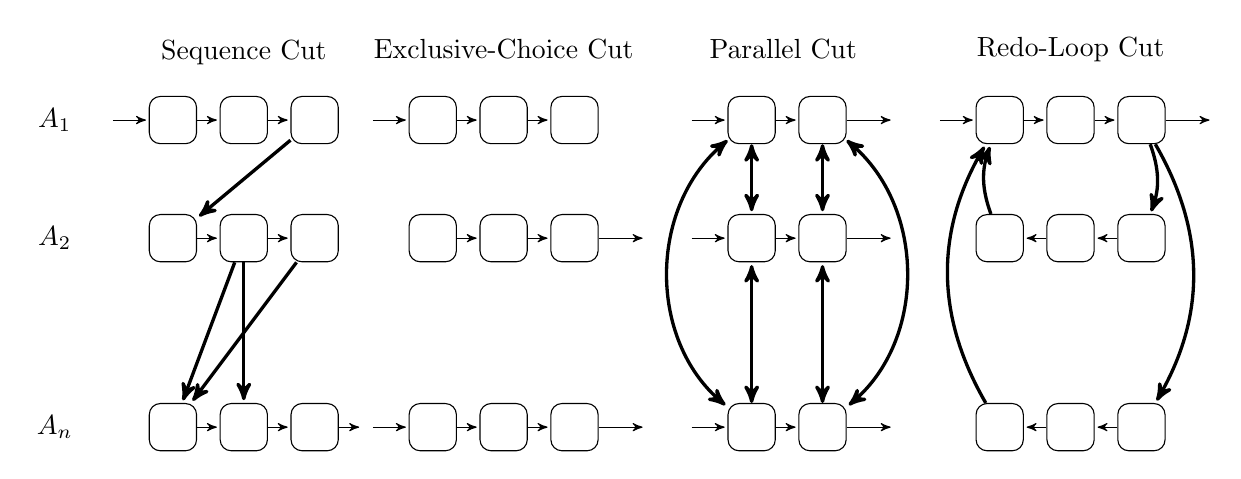
\begin{tikzpicture}[node distance = .9cm,,initial text = \textcolor{red}{},->]
        \node[]  (1000) []                  {$A_1$};
        \node[]  (2000) [below of=1000,node distance=1.5cm]     {$A_2$};
        \node[]  (x000) [below of=2000]     {};
        \node[]  (n000) [below of=x000,node distance=1.5cm]     {$A_n$};

        %% Sequence
        \node[activ,initial]  (1001) [right of=1000,node distance=1.5cm]    {};
        \node[activ]  (1002) [right of=1001]    {};
        \node[activ]  (1003) [right of=1002]    {};
        \node[]       (t002) [above of=1002,yshift=-0.05cm]    {Sequence Cut};
        \path   (1001) edge []   node {} (1002)
                (1002) edge []   node {} (1003);

        \node[activ]  (2001) [right of=2000,node distance=1.5cm]    {};
        \node[activ]  (2002) [right of=2001]    {};
        \node[activ]  (2003) [right of=2002]    {};
        \path   (2001) edge []   node {} (2002)
                (2002) edge []   node {} (2003);

        \node[activ]  (n001) [right of=n000,node distance=1.5cm]    {};
        \node[activ]  (n002) [right of=n001]    {};
        \node[activ]  (n003) [right of=n002]    {};
        \coordinate[right of=n003,xshift=-0.3cm] (n003e);
        \path   (n001) edge []   node {} (n002)
                (n002) edge []   node {} (n003)
                (n003) edge []   node {} (n003e);

        %% Exclusive
        \node[activ,initial]  (1004) [right of=1003,node distance=1.5cm]    {};
        \node[activ]  (1005) [right of=1004]    {};
        \node[activ]  (1006) [right of=1005]    {};
        \node[]       (t005) [above of=1005]    {Exclusive-Choice Cut};
        \path   (1004) edge []   node {} (1005)
                (1005) edge []   node {} (1006);

        \node[activ]  (2004) [right of=2003,node distance=1.5cm]    {};
        \node[activ]  (2005) [right of=2004]    {};
        \node[activ]  (2006) [right of=2005]    {};
        \coordinate[right of=2006] (2006e);
        \path   (2004) edge []   node {} (2005)
                (2005) edge []   node {} (2006)
                (2006) edge []   node {} (2006e);

        \node[activ,initial]  (n004) [right of=n003,node distance=1.5cm]    {};
        \node[activ]  (n005) [right of=n004]    {};
        \node[activ]  (n006) [right of=n005]    {};
        \coordinate[right of=n006] (n006e);
        \path   (n004) edge []   node {} (n005)
                (n005) edge []   node {} (n006)
                (n006) edge []   node {} (n006e);

        %% Parallel
        \node[activ,initial]  (1007) [right of=1006,node distance=2.25cm]    {};
        \node[activ]  (1009) [right of=1007]    {};
        \node[]       (t008) [above of=1009,xshift=-0.5cm]    {Parallel Cut};
        \coordinate[right of=1009] (1009e);
        \path   (1007) edge []   node {} (1009)
                (1009) edge []   node {} (1009e);

        \node[activ,initial]  (2007) [right of=2006,node distance=2.25cm]    {};
        \node[activ]  (2009) [right of=2007]    {};
        \coordinate[right of=2009] (2009e);
        \path   (2007) edge []   node {} (2009)
                (2009) edge []   node {} (2009e);

        \node[activ,initial]  (n007) [right of=n006,node distance=2.25cm]    {};
        \node[activ]  (n009) [right of=n007]    {};
        \coordinate[right of=n009] (n009e);
        \path   (n007) edge []   node {} (n009)
                (n009) edge []   node {} (n009e);

        %% Redo
        \node[activ,initial]  (1010) [right of=1009,node distance=2.25cm]    {};
        \node[activ]  (1011) [right of=1010]    {};
        \node[activ]  (1012) [right of=1011]    {};
        \node[]       (t011) [above of=1011]    {Redo-Loop Cut};
        \coordinate[right of=1012] (1012e);
        \path   (1010) edge []   node {} (1011)
                (1011) edge []   node {} (1012)
                (1012) edge []   node {} (1012e);

        \node[activ]  (2010) [right of=2009,node distance=2.25cm]    {};
        \node[activ]  (2011) [right of=2010]    {};
        \node[activ]  (2012) [right of=2011]    {};
        \path   (2011) edge []   node {} (2010)
                (2012) edge []   node {} (2011);

        \node[activ]  (n010) [right of=n009,node distance=2.25cm]    {};
        \node[activ]  (n011) [right of=n010]    {};
        \node[activ]  (n012) [right of=n011]    {};
        \path   (n011) edge []   node {} (n010)
                (n012) edge []   node {} (n011);

        \path   [very thick]
                (1003) edge []  node {} (2001)
                (2002) edge []  node {} (n001)
                (2003) edge []  node {} (n001)
                (2002) edge []  node {} (n002);

        \path   [very thick]
                (1007) edge [<->]  node {} (2007)
                (1009) edge [<->]  node {} (2009)
                (n007) edge [<->]  node {} (2007)
                (n009) edge [<->]  node {} (2009)
                (1007) edge [bend right=50,<->]  node {} (n007)
                (1009) edge [bend left=50,<->]  node {} (n009);

        \path   [very thick]
                (1012) edge [bend left=20]  node {} (2012)
                (1012) edge [bend left]  node {} (n012)
                (2010) edge [bend left=20]  node {} (1010)
                (n010) edge [bend left]  node {} (1010);
    \end{tikzpicture}
\end{center}

The Inductive Miner algorithm has some nice properties: The resulting model is sound, has perfect fitness, and can handle infrequent or incomplete behaviour.

\section{Conformance Checking}

\emph{Conformance checking} is all about verifying that a model fits the data.
We have three main use cases: Compliance checking (detecting fraud etc.), verifying process discovery results, and checking for conformance to a specification.

\subsection{Causal footprints}

\begin{minipage}[t]{0.6\textwidth}
    This method compares the footprint of the event log and the footprint of the model.
    We can calculate a value for the \emph{footprint-based conformance} by dividing the number of matches between the footprints by the overall number of activity pairs.
\end{minipage}%
\begin{minipage}[t]{0.4\textwidth}
    \[ \frac{\abs{\text{same footprint entries}}}{\abs{\text{activities}}^2} \]
\end{minipage}

\vspace{-0.5\baselineskip}
\subsection{Token Replay}

\emph{Token replay} measures fitness of a model as a proportion of behaviour in the event log according to the model.
Formally, we calculate this value by executing our (WF-net $N$) model on a trace $\sigma$ and tracking four values:
\begin{itemize}
    \item $p$: Number of produced tokens,
    \item $c$: Number of consumed tokens,
    \item $m$: Number of missing tokens (consumed, but not actually existing),
    \item $r$: Number of remaining tokens (produced, but not consumed).
\end{itemize}

The fitness is then defined as:
$
    fitness(\sigma, N) = \frac{1}{2} \left( 1 - \frac{m}{c} \right) + \frac{1}{2} \left( 1 - \frac{r}{p} \right)
$

To compute the fitness for an entire log, simply track the respective sums of all four values for each trace in the log.

Token replay imposes an important restriction on the fitness value: It is limited by the notation of the model (WF-nets).
Therefore token replay cannot be used to measure conformance of models with silent transitions or models with two transitions with the same label.

\vspace{-0.5\baselineskip}
\subsection{Alignment-based Conformance Checking}

\emph{Alignment-based conformance checking} is more general than token replay and measures, as the name implies, \emph{alignments}.

\begin{halfboxl}
An \emph{alignment} is a pair of sequences of moves.
Moves are either transitions or the ``no move'' symbol $\gg$.
Both move sequences in the alignment should be equal ignoring $\gg$ symbols.
The first move sequence corresponds to a trace in the event log, the second one to a run of the model.
\end{halfboxl}%
\begin{halfboxr}
\vspace{-\baselineskip}
\begin{center}
\begin{tabular}{c|c|c|c|c}
a & b & b & b & $\gg$ \\ \hline
a & b & $\gg$  & b & a
\end{tabular}

An example alignment with a $\gg$ in both move sequences that aligns $abbb$ and $abba$. \\
It is not unique.
\end{center}
\end{halfboxr}

Many metrics are possible to compute the fitness of an alignment.
The \emph{standard cost function} simply counts the number of $\gg$ symbols in an alignment.
Of course this means that many optimal alignments are possible with this metric.

\section{Decision Mining}

Decision mining can use data-aware petri-nets to give a more detailed model with conditions (\emph{guards}) at transitions at so-called \emph{decision points}.
Decision points are the places in networks with multiple outgoing transitions.
Decision trees can be used to find these conditions: Use the next activity as the response variable and, for example, attributes of the previous activities as the predictor variables.

\section{Organisational Mining}

\subsection{Resource-activity Matrix}

\begin{halfboxl}
The \textit{resource-activity matrix} provides information as to which of the involved employees performs which activities how often. To compute it, one looks at each \((resource, \: activity)\)-pair, computes how often it comes up in the log and divides it by the number of traces.

\[\frac{instances \: of \: a_i \: performed \: by \: resource \: r_j}{amount \: of \: traces}\]
\end{halfboxl}%
\begin{halfboxr}
\vspace{-\baselineskip}
\begin{align*}
    & \langle a_1^{r_1} \rangle \\
    & \langle a_2^{r_3},a_3^{r_4} \rangle \\
\end{align*}
\[\begin{array}{c|c|c|c|c}
        & a_1   & a_2   & a_3   & a_4   \\ \hline
    r_1 & 0.5   & 0     & 0     & 0     \\ \hline
    r_2 & 0     & 0     & 0     & 0     \\ \hline
    r_3 & 0     & 0.5   & 0     & 0     \\ \hline
    r_4 & 0     & 0     & 0.5   & 0     \\
\end{array}\]
\end{halfboxr}

As an example, on the right, we have a log, and below we have its resource activity matrix. What it says is that $r_1$ performs $a_1$ on average once every two traces, and that $r_3$ and $r_4$ respectively perform $a_2$ and $a_3$ on average every two traces.

\subsection{Social Networks}

\begin{halfboxl}
\paragraph{Handover of work Matrix} The \textit{handover of work matrix} provides information as to which employees transfer work to which other employees. To compute it, you need a process model in the form of a petri net.

On the right we have a petri net for the log shown above. This is important as handover of work only happens between successive activities, and especially not between concurrent activities.
\end{halfboxl}%
\begin{halfboxr}
\vspace{-\baselineskip}
    \begin{center}
        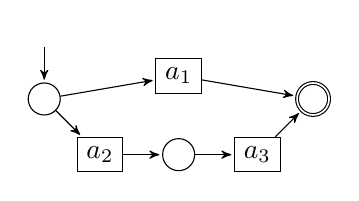
\begin{tikzpicture}[->]
            \node[initial,place, initial where=above]    (0) []                  {$\;$};
            \node[trans]            (1) [below right of=0]  {$a_2$};
            \node[place]            (2) [right of=1]        {$\;$};
            \node[trans]            (3) [right of=2]        {$a_3$};
            \node[accepting,place]  (4) [above right of=3]  {$\;$};
            \node[trans]            (5) [above of=2]        {$a_1$};

            \path   (0) edge []   node {} (1)
                    (1) edge []   node {} (2)
                    (2) edge []   node {} (3)
                    (3) edge []   node {} (4)
                    (0) edge []   node {} (5)
                    (5) edge []   node {} (4);
        \end{tikzpicture}
    \end{center}
    \[\begin{array}{c|c|c|c|c}
        & r_1   & r_2   & r_3   & r_4   \\ \hline
    r_1 & 0     & 0     & 0     & 0     \\ \hline
    r_2 & 0     & 0     & 0     & 0     \\ \hline
    r_3 & 0     & 0     & 0     & 0.5   \\ \hline
    r_4 & 0     & 0     & 0     & 0     \\
\end{array}\]
\end{halfboxr}

What we see in this matrix is that once every two cases on average, $r_3$ hands over work to $r_4$. This would not be the case for example if we had a model in which $a_2$ and $a_3$ were concurrent.

\begin{halfboxl}
To compute this matrix, use the formula on the right for each ordered pair $(r_i,r_j)$. The corresponding graph can be found on the next page.
\end{halfboxl}%
\begin{halfboxr}
\vspace{-5pt}
\[\frac{times \; r_i \; hands \; over \; work \; to \; r_j}{amount \; of \; traces \; in \; log}\]
\end{halfboxr}

\begin{halfboxl}
\paragraph{Subcontracting matrix} The \textit{subcontracting matrix} provides information about which employees outsource work to other employees before taking back control.

In the log on the right, you have $r_3$ outsourcing work to $r_4$. That is, $r_4$ executes an activity between two activities from $r_3$. To compute the matrix, for each ordered pair $(r_i,r_j)$, compute the formula on the right.
\paragraph{Working Together Matrix} The \textit{working together matrix} indicates how much employees cooperate on cases.
For example, on the right, you have $r_1$, $r_3$ and $r_4$ working together. To compute the matrix, compute for each pair $(r_i,r_j)$ the formula on the right.
\paragraph{Social Network Graph} Any of these matrices can be turned into \textit{social network graphs} by using the resources as nodes and non-zero matrix entries as edges with their value as a tag. (note: you might have a lower threshold to prune outliers)
\end{halfboxl}%
\begin{halfboxr}
\[\langle a_2^{r_3},a_3^{r_4},a_4^{r_3} \rangle\]
\vspace{30pt}
\[\frac{times \; r_i \; outsources \; work \; to \; r_j}{amount \; of \; traces \; in \; log}\]
\vspace{20pt}
\[\langle a_2^{r_3},a_3^{r_4},a_4^{r_1} \rangle\]
\vspace{20pt}
\[\frac{traces \; in \; which \; r_i \; and \; r_j \; both \; work}{amount \; of \; traces \; in \; log}\]
\vspace{15pt}
\begin{center}
    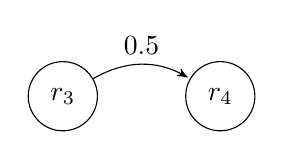
\begin{tikzpicture}[->, node distance=2cm]

        \node[state]    (0) []              {$r_3$};
        \node[state]  (1) [right of=0]              {$r_4$};

        \path   (0) edge [bend left]   node {$0.5$} (1);
    \end{tikzpicture}
\end{center}
\end{halfboxr}


\vspace{-\baselineskip}
\section{Process Mining Framework}

\emph{Pre mortem event data} is data about cases that are still running, while \emph{post mortem data} is only about dead cases.

\subsection{Refined Process Mining Framework}

\begin{enumerate}
    \item \emph{Cartography}: Process models as maps
        \begin{enumerate}
            \item \emph{Discover}: Find process models.
            \item \emph{Enhancer}: Extend/repair models with event logs.
            \item \emph{Diagnose}: Analyse models without event logs.
        \end{enumerate}
    \item \emph{Auditing}: Confronting model and reality
        \begin{enumerate}
            \item \emph{Detect}: Using the models, find violations of current real-world rules of currently running cases (pre mortem).
            \item \emph{Check}: Find weird behavior in the model (deviations, compliance).
            \item \emph{Compare}: On post mortem data, find deviations of current rules.
            \item \emph{Promote}: Create new rules from the models.
        \end{enumerate}
    \item \emph{Navigation}: Supporting process execution
        \begin{enumerate}
            \item \emph{Explore}: Explore currently running processes using current data and models.
            \item \emph{Predict}: Predict facts like runtime or success probability for running cases.
            \item \emph{Recommend}: Recommend good choices for current cases.
        \end{enumerate}
\end{enumerate}

\emph{Operational support}, that is supporting current cases, is is done by the Detect, Predict and Recommend actions.

\subsection[L* Lifecycle for Process Mining]{$L^\ast$ Lifecycle Model for Process Mining}

\begin{enumerate}[leftmargin=60pt]
    \item[\emph{Stage 0 --}] \emph{Plan and justify}: Plan the project and justify the project. Is the project data-driven, question-driven or goal-driven?
    \item[\emph{Stage 1 --}] \emph{Extract}: Actually get some event data.
    \item[\emph{Stage 2 --}] \emph{Create control-flow model}: Find a control-flow model for the available data. Use conformance checking and alignments.
    \item[\emph{Stage 3 --}] \emph{Create integrated process model}: Replay the event data on the control-flow model to learn about e.g.\ time, data, resources. Merge this into a greater model.
    \item[\emph{Stage 4 --}] \emph{Operational support}: Use the model for detection, predictions and recommendations (operational support). This only works for structured processes (``Lasagna processes'').
\end{enumerate}

\subsection{Mining Spaghetti Processes}

Because spaghetti processes are less structured than lasagna processes, we need to focus on some subset of the data.
\begin{itemize}
    \item \emph{Subset of activities}: E.g.\ most frequent, or some region.
    \item \emph{Subset of cases}: Choose a homogenous group of cases (by doing clustering, for example), or subclasses.
    \item \emph{Subset of paths}: E.g.\ most frequent.
\end{itemize}

\section{Big Event Data}

{\tiny ProTip: Use MongoDB, it's web scale. Because it uses sharding. And has no joins.}

We distuingish \emph{data warehouses}, containing structured and cleaned up data, from \emph{data lakes}, which contain unstructured data.

Very large amounts of event data may be too large to be saved, so a \emph{streaming} approach is useful: Using algorithms that do not need the complete event log, but process a stream.

Another way to make event logs smaller is by \emph{decomposition}.
This can be done on activities, or on cases, whatever makes most sense in the application context.
Conformance checking and Discovery (if it's only counting) can be easily decomposed on a case-level and distributed, but activity-based distribution is usually harder.

This decomposition can be done with \emph{MapReduce}: Worker nodes apply a \texttt{map} function to each datum (e.g.\ case).
The output is a collection of key-value pairs.
The \emph{shuffle} phase redistributes data so that pairs with the same key end up at the same worker.
Then, a \texttt{reduce} function is used that processes each group.

One can refer to a decomposition of an event log as a \emph{process cube}, because events are split along some axes into (hyper-)cubes.
A comparison between cubes and e.g.\ their models is called \emph{comparative process mining}.

\end{document}
